%TC: macro \marginfootnote [other]
%TC: envir SCfigure [] other
%TC: macrocount beginSCfigure [figure]
\documentclass[11pt,twoside]{report}
\usepackage{preamble}
\setcounter{chapter}{6}
\graphicspath{{../img/}}

\begin{document}
\chapter{Drying kinetics and nucleation of aerosol droplets}

\section{Introduction}

We have concentrated on the problem of modelling hard spheres at high densities, with a paritcular focus on supercooled liquids and glasses.
Another problem at high densities is crystal nucleation.
In this chapter we will address a practical application of nucleation: nucleation of salt crystals insdide of aerosol droplets, with applications to climate modelling and industrial spray drying.
We will describe these applications in more detail below.

One of the leading known-unknowns in climate modelling is the contribution to the greenhouse effect; salt droplets have different refractive properties depending on whether they are in crystal or liquid states which has an impact on the indirect effect.
Understanding the nucleation rates of droplets in the troposphere is thus potentially a crucial ingredient in climate science.
In order to keep statistical physicists alive long enough to reach a consensus on the nature of the glass transition, we have a fervent interest in better descriptions of the climate to inform policy.
\todo{Add something about industrial spray drying}

We briefly review the nucleation problem below starting from the mean field description.
Above the freezing point the crystal is the thermodynamically stable phase, so mean field (Landau) descriptions start by positing the lower free energy of the crystal phase in this regime.
In mean field, where fluctuations are impossible, transitioning from one phase to another is impossible however.
In physical dimensions (finite $d$) first-order phase transitions are kinetically allowable through fluctuations: classical nucleation theory describes how one thermodynamically extends the mean field (Landau) description to allow for fluctuations with a single reaction coordinate.
We describe this framework in \ref{sec:classical-nucleation-theory}

Nucleation rates of salt solutions are a much harder problem than hard spheres, a toy system, so our microscopic morphometric formalism will be unlikely to work here at present.
In stead we will start from the other mesoscale limit, where the droplet can be treated as a continuum.
At present real systems are too complex to be treated from first principles, so we will employ phenomenological fits to available data assuming classical nucleation theory.
We hope one day theory will allow a connection between microscopic and mesoscopic approaches, paving the way to a properly first-principles treatment of real systems.

\section{Experiments}

We describe the experiments here, carried out by the Gregson in the Reid group.
I did not contribute to this work, but it is essential to understand their setup as my work attempts to model their data.

They levitate droplets in a humidity controlled environment.
The humidity control consists of air currents which they can control the water in.
They can turn off the water at any point to rapidly switch between different humidities.
They place a salt crystal inside the apparatus, and set the humidity high to grow a droplet.
The water wets the crystal, dissolving the salt and becoming a solution.
When they want to study drying they turn off the water flow (or turn it down) so water starts to evaporate and it dries.
After the droplet is highly saturated by the salt nucleation occurs, with the experimental observation that it occurs disproportionately at the boundary.

The droplet is monitored by scattering light.
When the scattering profile goes haywire (coalesces) this indicates that the droplet has nucleated.
Nucleation and growth occur on such a short time scale that it is not possible to obtain information on where inside the droplet this occurs or how many initial nucleation sites there were, only that the droplet has crystallised.
Nucleation seemed to occur where the average concentration of salt inside the droplets was not very supersaturated (and thus nucleation is not expected), suggesting that an inhomogeneous profile might be driving it.
Fast water evaporation rates for dry conditions would lead to a build up of salt at the boundary.
This scenario is more akin to spray drying than climate modelling.
Follow up experiments by the Reid group placed the droplets inside scanning electron microscopes (SEM) for imaging.
These find that in general for \ce{NaCl} the nucleation does seem to occur at the boundary in line with this hypothesis.
\marginfootnote{I am reversing chronology here.
  Actually we used our numerical model to predict this first, and later the SEM experiments were performed which confirmed this.}
The experiments featuring slower evaporation tend to have more perfect crystals, suggesing a fewer number of nucleation sites and allowing for slow crystal growth.
The SEM results for \ce{NaNO3} are inconclusive, although the resulting crystal is more spherical suggesting multiple nucleation sites/less strongly distributed at the boundary.

While there is an air-water interface, this phase boundary is not believed to act as a heterogeneous nucleation sites; rather the increased concentration of salt at the boundary drives it (we conjecture this).
They use fancy distilled water to eliminate potential heterogeneous nucleation sites due to impurities.
We will attempt to model the nucleation as homogeneous nucleation, albeit with an inhomogeneous evolving concentration profile.
As such we need to model:
\begin{itemize}
  \item The instantaneous homogeneous nucleation rates for a given concentration profile.
  \item The rate of evaporation of water from the droplet.
  \item The evolution of the concentration inside the droplet.
\end{itemize}

We have the following experimental datasets for \ce{NaNO3}, RH = relative humidity
\begin{itemize}
\item Varying temperature at constant RH=0 (dry conditions).
\item Varying Initial solute concentration at constant $T$=20\si{K}
\item Varying gas RH at constant $T$=20\si{K}.
\end{itemize}

\section{Notation}

We consider a droplet of radius $R(t)$ and consider concentration profiles at position $\vec{r}$ inside the droplet.
We will later assume spherical symmetry and reduce the dependance on $\vec{r}$ to a dependance on the distance from the centre $r = |\vec{r}|$.
The droplet consists of a binary fluid, with solute and solvent (mass) concentration profiles labelled $\rho^{(s)}(\vec{r})$ and $\rho^{(f)}(\vec{r})$ respectively.
The mass fraction of each component is written
\begin{equation}\label{eq:mass-fraction}
  Y^{(i)}(\vec{r}) = \frac{\rho^{(i)}(\vec{r})}{\sum_j \rho^{(j)}(\vec{r})} = \frac{\rho^{(i)}(\vec{r})}{\rho^{(f)}(\vec{r}) + \rho^{(s)}(\vec{r})} \qquad i \in \{f, s\}
\end{equation}
Clearly $Y^{(f)} = 1 - Y^{(s)}$ as they must sum to unity, so we can choose either to describe the fluid;
we will henceforth use solute mass fraction $Y^{(s)}$.
The density of the droplet is
\begin{equation}
  \rho(\vec{r}) = \sum_i \rho^{(i)}(\vec{r}) = \rho^{(f)}(\vec{r}) + \rho^{(s)}(\vec{r}) = \frac{\rho^{(s)}(\vec{r})}{\rho^{(s)}(\vec{r})},
\end{equation}
but $\rho^{(s)}$ and $Y^{(s)}$ are related by an equation of state so we could equivalently write:
\begin{equation}
  \rho(\vec{r}) =
  \frac{\rho^{(s)}(\vec{r})}{Y^{(s)}(\rho^{(s)}(\vec{r}))} =
  \frac{\rho^{(s)}(Y^{(s)}(\vec{r}))}{Y^{(s)}(\vec{r})}.
\end{equation}
Volume additivity holds to a good approximation \cite{Handscomb???}, i.e.\ the density and concentrations are related by
\begin{equation}\label{eq:volume-additivity}
  \begin{aligned}
    \frac{1}{\rho} &=
    \sum_{k \in \{f,s\}} \frac{Y^{(k)}}{\rho^{(j)}_0} \\
    &=
    \frac{Y^{(i)}}{\rho^{(i)}_0} +
    \frac{1 - Y^{(i)}}{\rho^{(j)}_0}
    \qquad i,j \in \{f,s\}, \; j \ne i.
  \end{aligned}
\end{equation}
means
(define)
\begin{equation}\label{eq:density-lambda}
  \begin{aligned}
    \Lambda^{(i)} &=
    \frac{1}{\rho^2} \frac{\partial \rho}{\partial Y^{(i)}} \\
    &=
    \frac{1}{\rho^{(i)}_0} -
    \frac{1}{\rho^{(j)}_0}
    \\
    &=
    \frac{\rho^{(j)}_0 - \rho^{(i)}_0}{\rho^{(i)}_0\rho^{(j)}_0}
    \qquad i,j \in \{f,s\}, \; j \ne i.
  \end{aligned}
\end{equation}
From \eqref{eq:volume-additivity} and \eqref{eq:density-lambda} we have
\begin{equation*}
  \begin{aligned}
    \frac{1}{\rho} &=
    \Lambda^{(i)} Y^{(i)} + \frac{1}{\rho^{(j)}_0} \\
    &=
    \Lambda^{(i)} \frac{\rho^{(i)}}{\rho} + \frac{1}{\rho^{(j)}_0}
    \qquad i,j \in \{f,s\}, \; j \ne i,
  \end{aligned}
\end{equation*}
which rearranges to give
\begin{equation*}
  (1 - \rho^{(i)} \Lambda^{(i)})
  \frac{1}{\rho} =
  \frac{1}{\rho^{(j)}_0}
  \qquad i,j \in \{f,s\}, \; j \ne i,
\end{equation*}
and finally we have
\begin{equation}
  \rho =
  \rho^{(j)}_0 (1 - \rho^{(i)} \Lambda^{(i)})
  \qquad i,j \in \{f,s\}, \; j \ne i.
\end{equation}
This means
\begin{equation}
  \begin{aligned}
    \rho - \rho^{(i)} &=
    \rho^{(j)}_0 (1 - \rho^{(i)} \Lambda^{(i)}) - \rho^{(i)} \\
    &=
    \rho^{(j)}_0 - \rho^{(i)}(1 + \rho^{(j)}_0 \Lambda^{(i)})
    \qquad i,j \in \{f,s\}, \; j \ne i.
  \end{aligned}
\end{equation}
or more importantly
\begin{equation}
  \frac{\rho^{(i)}}{\rho} =
  \frac{\rho^{(i)}}{\rho^{(j)}_0 (1 - \rho^{(i)} \Lambda^{(i)})}
  \qquad i,j \in \{f,s\}, \; j \ne i.
\end{equation}
Note:
\begin{equation*}
  \Lambda^{(f)} = -\Lambda^{(s)}.
\end{equation*}

\begin{SCfigure}[H]
  \missingfigure[figwidth=\linewidth]{}
  \caption{The model droplet: we have a liquid phase and a vapour phase separated by a moving boundary at radius $r=R(t)$.
  We have a shrinking boundary $\dot{R} < 0$ for drying.}
\end{SCfigure}

\section{Nucleation model}
\subsection{Classical nucleation theory}
\label{sec:classical-nucleation-theory}

Numerical values taken from capilliary paper.

Here we review classical nucleation theory (CNT) which describes the mechanism of first-order transitions by modelling the formation of the new phase as fluctuations inside a metastable phase.
We imagine the metastable phase to have `equilibrated' in the sense that it has sampled all of the microstates corresponding to the metastable-phases macrostate, so that fluctuations can be treated as Boltzmann-weighted fluctuations.
This allows a thermodynamic description of nucleation, and is widely used/confirmed by simulation/experimental studies \cite{?}.
We loosely follow the excellent review of Sears \cite{Sears?}.

Consider a small region of the new phase forms inside the metastable one, and we wish to calculate the (free) energetic cost of this formation.
The region has a smaller chemical potential due to this new phase being the thermodynamic ground state, however it also introduces a phase-boundary at the edge of this region paying a surface energy penalty.
This gives the energy change (Gibbs)
\begin{equation}
  \Delta G(R) = \gamma A - |\Delta \mu| \rho_s V
\end{equation}
where $\Delta \mu$ is the different in chemical potential between the two phases and we have written it with absolute bars to make the sign explicit, $A$ and $V$ are the surface areas and volumes of the new region.
Note that this is equivalent to the reversible work to assemble such a system, so in principle this could be calculated via the formalism described in previous chapters (at least for hard spheres where we have shown this is accurate).
Assuming the region to be spherical of radius $R$ this reduces to the single reaction coordinate
\begin{equation}
  \Delta G(R) = 4\pi R^2 \gamma - \frac{4}{3} \pi R^3 \rho_s |\Delta \mu|
\end{equation}
The maximum of this equation is thus the thermodynamic barrier to nucleation.
Defining $\Delta G^{*} = \max{(\Delta G)}$ and $R^{*} = \argmax{(\Delta G)}$ we have
\begin{align}\label{eq:cnt-barrier}
  \Delta G^{*} &= \frac{4}{3} \pi (R^{*})^2 \gamma \\
  (R^{*}) &= -\frac{2\gamma}{\rho_s \Delta\mu}
\end{align}
In the above we assumed the new region is spherical, but in general it could be of arbitrary (but compact) shape and it is possible for there to be multiple reaction coordinates leading to novel nucleation kinetics.
In the latter case a simple CNT description would break down.

From \eqref{eq:cnt-barrier} we write the homogeneous nucleation rate per unit volume as
\begin{equation}
  J = \kappa \exp{\left(-\frac{\Delta G^{*}}{k_B T}\right)}
\end{equation}
where $\kappa$ is a kinetic prefactor.
We will now describe the functional forms of these quantities within CNT, giving a phenomenological description of nucleation rates within CNT.

The chemical potential expressed in terms of mean ionic activity is
\begin{equation}
  \begin{aligned}
  \exp{-\frac{\Delta \mu}{k_B T}} &=
  \nu \ln{\left( \frac{a_\pm}{a_{0\pm}} \right)} \\
  &=
  \nu \ln{\left( \frac{\gamma_\pm}{\gamma_{0\pm}} \frac{m}{m_0} \right)}
  \end{aligned}
\end{equation}
$nu$ is sum of ions (2 for \ce{NaCl}), $a_\pm$ is mean ionic activity, $\gamma_\pm$ is mean ionic activity coefficient, $m$ and $m_0$ are molarities at equilibrium and crystal stabilisation respectively, ?%
\todo{Find out what $a_{0\pm}$ and $\gamma_{0\pm}$ are from Flo.}

A commonly used approximation for the kinetic prefactor in \eqref{?} is \cite{Sears?}:
\begin{align}
  \kappa &= \rho_l j Z \\
  j &\sim \rho_l D_l R^* \\
  Z &\sim (n^*)^{-\tfrac{2}{3}}
\end{align}
$\rho_l$ is liquid phase density, $j$ is rate of aggregation, $Z$ is Zeldovich factor, $n^*$ is excess number of molecules in critical nucleus (check references!).
\todo{Review the literatue on where this comes from.}

Inserting values from literature we see that the homogeneous nucleation rate per unit volume is essentially a step function for both \ce{NaCl} and \ce{NaNO3}.
We tried various values of surface tension for \ce{NaNO3}, however it did not specifically change the phenomenon.
\todo{2d plots of nucleation rates.}
The nucleation rates are weakly dependent on the temperature, and strongly dependent on the salt concentration.

The experimental data cannot directly give the nucleation rates per unit volume, rather they determine whether the entire droplet has crystallised; to make a comparison we have to go from the local nucleation rate to the entire droplet's rate.
In the next section we will describe this process based on Poisson statistics, and later we will present a diffusion-evaporation model for obtaining a trajectory of concentration profiles.

\subsection{Droplet nucleation rates}

We will assume Poisson statistics in order to determine the survival probabilty of the droplet, i.e.\ the probability that there has been no nucleation event.
This is mathematically identical to calculating e.g.\ decay rates of radioactive isotopes.

Suppose we have the instantaneous droplet concentration profile $\rho_s(r; t)$ at a certain point in time.
Assuming CNT from the previous section, we know the nucleation rate/unit volume everywhere in the droplet $J(r; t) = J\Big(\rho_s(r; t)\Big)$.
The total nucleation rate across the droplet, i.e.\ the number of expected events per second globally is:
\begin{equation}
  W = \int J dV
  = 4\pi \int_0^{R(t)} J(r; t) \, r^2 dr
\end{equation}
We treat the number of events in the volume element $r \to r + \Delta r$ Between $t \to t+\Delta t$ as a Poisson process, with mean events:
\begin{equation}
  \begin{aligned}
    \mu(r) &= \frac{4\pi}{3} \left( (r+\Delta r)^3 - r^3 \right)
    \int_t^{t+\Delta t} J(r,t') \, dt' \\
    &\simeq
    4\pi r^2 \Delta r J(r, t) \Delta t
  \end{aligned}
\end{equation}
For Poisson statistics the probability of having exactly $n$ events as
\begin{equation}
  P(n; r) = \frac{e^{-\mu(r)} \mu(r)^n}{n!}.
\end{equation}
Giving probability of no nucleation event (`survival') as $P(0; r) = e^{-\mu(r)}$.
This gives the probability of having seen no events across the whole droplet in this time period as:
\begin{equation}
  \begin{aligned}
    \textrm{Prob}\left[ \textrm{no event in } t \to t + \Delta t \right]
    &=
    \exp{\left(
      -4\pi \int_t^{t+\Delta t} dt' \int_0^{R(t')} dr r^2 J(r, t')
      \right)}
    \\ &\simeq
    \prod_i \exp{\left(-4\pi (i\Delta r)^2 J(i\Delta r) \Delta t \Delta r\right)}
  \end{aligned}
\end{equation}
where the latter line is a useful approximation for numerical descriptions on a uniformly separated discrete grid.

\subsection{Inverse problem}

We can try to determine the nucleation rates directly from experiments by observing the stochastic nucleation behaviour over repeat trajectories and comparing these against the numerical model.
In this way we can attempt to find $J$ as a function of concentration directly from the known survival probabilities; this is an inverse problem and is in general not well posed.
We can make some progress by making some strong assumptions about the form of $J$ based on physical intuition.
We will then test for self-consistency to justify this approach ad-hoc.

We generally expect nucleation to occur at the surface $r = R$ where the concentration is most saturated.
We therefore expect $J = J(\rho^{(s)}(R), T)$.
We thus expect the survival probability \eqref{eq?} to be dominated by a term like
\begin{equation}
  \textrm{Prob}\left[ \textrm{no event in } t \to t + \Delta t \right]
  \sim
  \exp^{-4\pi R^2 \Delta t J(R) \xi}
\end{equation}
where $\xi$ is some lengthscale over which the concentration is enriched i.e.\ where nucleation occurs.
Assuming that $\xi$ will be the same at all state points, we can determine $J \xi$ by fitting it against the nucleation rates seen in the lab.

\section{Diffusion model for a drying droplet}

\subsection{Evolution equations}

To determine the concentration profile trajectory for a drying droplet we have to consider the relative motion of solute-solvent species inside the droplet, the relative motion of various species in the vapour phase, as well as the evaporation of solvent across the phase boundary.
This problem reduces to a moving boundary problem with diffusion.

Starting from conservation of mass/species we have the continuity equations
\begin{subequations}
\begin{align}
  \label{eq:total-continuity}
  \frac{\partial \rho}{\partial t} +
  \vec{\nabla} \cdot (\rho \vec{v}) &= 0 \\
  \label{eq:species-continuity}
  \frac{\partial \rho^{(i)}}{\partial t} +
  \vec{\nabla} \cdot (\rho^{(i)} \vec{v}^{(i)}) &= 0
  \qquad i \in \{f,s\}
\end{align}
\end{subequations}
where $\vec{v}^{(i)}$ is the velocity of species $i$ and the mass-averaged fluid velocity is
\begin{equation}
  \vec{v} = \sum_i Y^{(i)} \vec{v}^{(i)}
\end{equation}
We have
\begin{equation*}
  \frac{\partial \rho^{(i)}}{\partial t} +
  \vec{\nabla} \cdot (\rho^{(i)} \vec{v}) +
  \vec{\nabla} \cdot (\rho^{(i)} (\vec{v}^{(i)} - \vec{v})) = 0
  \qquad i \in \{f,s\}
\end{equation*}
and defining the relative mass flux as
\begin{equation}\label{eq:relative-mass-flux}
  \vec{j}^{(i)} = \rho^{(i)} (\vec{v}^{(i)} - \vec{v})
  \qquad i \in \{f,s\}
\end{equation}
gives
\begin{equation}\label{eq:species-continuity-relative}
  \frac{\partial \rho^{(i)}}{\partial t} +
  \vec{\nabla} \cdot (\rho^{(i)} \vec{v}) +
  \vec{\nabla} \cdot \vec{j}^{(i)} = 0
  \qquad i \in \{f,s\}
\end{equation}

Note that the divergence term in spherical coordinates is
\begin{equation*}
  \vec{\nabla} \cdot \vec{j} =
  \frac{1}{r^2} \frac{\partial (r^2 \rho u)}{\partial r}
\end{equation*}

\subsection{Liquid phase analysis I: mass fraction}

Assume Fick's law for diffusion:
\begin{equation}\label{eq:ficks-law}
  \vec{j}^{(i)} = -D_{\textrm{eff}} \rho \vec{\nabla} Y^{(i)}
\end{equation}
where $D_{\textrm{eff}}$ is an effective \emph{binary} diffusion constant for the relative motion.
Note that as $Y^{(f)} + Y^{(s)} = 1$ we have
\begin{equation*}
  \vec{j}^{(i)} = -\vec{j}^{(i)}
\end{equation*}

Expressing the concentration terms in the species equation in terms of the density and mass fraction gives
\begin{align*}
  \frac{\partial \rho^{(i)}}{\partial t} &=
  \frac{\partial (\rho Y^{(i)})}{\partial t} \\
  &=
  \rho \frac{\partial Y^{(i)}}{\partial t} +
  Y^{(i)} \frac{\partial \rho}{\partial t} \\
  &=
  \rho \frac{\partial Y^{(i)}}{\partial t} -
  Y^{(i)} \vec{\nabla} \cdot (\rho \vec{v})
\end{align*}
and
\begin{equation*}
  \begin{aligned}
    \vec{\nabla} \cdot (\rho^{(i)} \vec{v}) &=
    \vec{\nabla} \cdot (\rho Y^{(i)} \vec{v}) \\
    &=
    \rho \vec{v} \cdot \vec{\nabla} Y^{(i)} +
    Y^{(i)} \vec{\nabla} \cdot (\rho \vec{v})
  \end{aligned}
\end{equation*}
Inserting these expressions into the species equation gives
\begin{equation}\label{eq:advection-continuity-1}
  \begin{aligned}
    \frac{\partial \rho^{(i)}}{\partial t} -
    \vec{\nabla} \cdot (\rho^{(i)} \vec{v}) +
    \vec{\nabla} \cdot \vec{j}^{(i)} &= \\
    \rho \frac{\partial Y^{(i)}}{\partial t} -
    Y^{(i)} \vec{\nabla} \cdot (\rho \vec{v}) +
    \rho \vec{v} \cdot \vec{\nabla} Y^{(i)} +
    Y^{(i)} \vec{\nabla} \cdot (\rho \vec{v}) +
    \vec{\nabla} \cdot \vec{j}^{(i)} &= \\
    \rho \left(
    \frac{\partial Y^{(i)}}{\partial t} +
    \vec{v} \cdot \vec{\nabla} Y^{(i)}
    \right) +
    \vec{\nabla} \cdot \vec{j}^{(i)}
    &= 0 \qquad i \in \{f,s\}
  \end{aligned}
\end{equation}
Thus inserting \eqref{eq:ficks-law} into \eqref{eq:advection-continuity-1} gives the mass fraction form of \eqref{eq:species-continuity-relative} as
\begin{equation}\label{eq:mass-fraction-continuity}
  \rho \left(
  \frac{\partial Y^{(i)}}{\partial t} +
  \underbrace{\vec{v} \cdot \vec{\nabla} Y^{(i)}}_\textrm{advection}
  \right)
  -
  \underbrace{\vec{\nabla} \cdot (D_{\textrm{eff}} \rho \vec{\nabla} Y^{(i)})}_\textrm{diffusion}
  = 0
  \qquad i \in \{f,s\}.
\end{equation}
Note: we only need solve this for a single component, e.g.\ for $i=s$, and then we have the other one through $Y^{(f)} + Y^{(s)} = 1$.
We must deduce the form of the fluid velocity $\vec{v}$ to close this equation.

Using the fact that $\rho = \rho(Y^{(i)})$, i.e.\
\begin{equation*}
  \frac{\partial \rho}{\partial t} =
  \frac{\partial \rho}{\partial Y^{(i)}} \frac{\partial Y^{(i)}}{\partial t}
\end{equation*}
transforms the continuity equation \eqref{eq:total-continuity} as
\begin{equation}\label{eq:advection-continuity-2}
  \begin{aligned}
    \frac{\partial \rho}{\partial t} +
    \vec{\nabla} \cdot (\rho \vec{v})
    &=
    \frac{\partial \rho}{\partial Y^{(i)}} \frac{\partial Y^{(i)}}{\partial t} +
    \vec{v} \cdot \vec{\nabla} \rho +
    \rho \vec{\nabla} \cdot \vec{v} \\
    &=
    \frac{\partial \rho}{\partial Y^{(i)}}
    \left(
    \frac{\partial Y^{(i)}}{\partial t} +
    \vec{v} \cdot \vec{\nabla} Y^{(i)}
    \right) +
    \rho \vec{\nabla} \cdot \vec{v} \\
    &= 0
  \end{aligned}
\end{equation}
Equating the bracketed terms in \eqref{eq:advection-continuity-1} and \eqref{eq:advection-continuity-2} gives
\begin{equation}
  \vec{\nabla} \cdot \vec{v}
  =
  \frac{1}{\rho^2}
  \frac{\partial \rho}{\partial Y^{(i)}}
  \vec{\nabla} \cdot \vec{j}^{(i)}
\end{equation}
which must be inverted to find $\vec{v}$ to model the advection.
Integrating both sides we find
\begin{equation*}
  \int_{\mathbb{V}}
  \vec{\nabla} \cdot \vec{v}
  \, d^3|\vec{r}|
  =
  \int_{\mathbb{V}}
  \frac{1}{\rho^2}
  \frac{\partial \rho}{\partial Y^{(i)}}
  \vec{\nabla} \cdot \vec{j}^{(i)}
  \, d^3|\vec{r}|
\end{equation*}
and applying Stokes' theorem to the LHS gives
\begin{equation*}
  \int_{\partial \mathbb{V}}
  \vec{v} \cdot
  \, d^2\vec{S}
  =
  \int_{\mathbb{V}}
  \frac{1}{\rho^2}
  \frac{\partial \rho}{\partial Y^{(i)}}
  \vec{\nabla} \cdot \vec{j}^{(i)}
  \, d^3|\vec{r}|
\end{equation*}
Using \eqref{eq:density-lambda} we have
\begin{equation*}
  \begin{aligned}
  \int_{\partial \mathbb{V}}
  \vec{v} \cdot
  \, d^2\vec{S}
  &=
  \Lambda^{(i)}
  \int_{\mathbb{V}}
  \vec{\nabla} \cdot \vec{j}^{(i)}
  \, d^3|\vec{r}| \\
  &=
  \Lambda^{(i)}
  \int_{\partial \mathbb{V}}
  \vec{j}^{(i)} \cdot
  \, d^2\vec{S}
  \end{aligned}
\end{equation*}
i.e.\ we obtain
\begin{equation*}
  \int_{\partial \mathbb{V}}
  (\vec{v} - \Lambda^{(i)} \vec{j}^{(i)})
  \cdot \, d^2\vec{S}
  = 0
\end{equation*}
or in differential form
\begin{equation}
  \left.
  (\vec{v} - \Lambda^{(i)} \vec{j}^{(i)})
  \right|_{\partial \mathbb{V}}
  = 0
\end{equation}
As we could have drawn arbitrary boundaries inside the droplet, we have
\begin{equation}
  \vec{v} =
  \Lambda^{(i)} \vec{j}^{(i)} =
  -D_{\textrm{eff}} \Lambda^{(i)} \rho \vec{\nabla} Y^{(i)}
\end{equation}
The concentration species equation \eqref{eq:species-continuity-relative} becomes
\begin{equation}\label{eq:species-continuity-advection-corrected}
  \begin{aligned}
    0 &=
    \frac{\partial \rho^{(i)}}{\partial t} +
    \vec{\nabla} \cdot
    \left(
    \rho^{(i)} \vec{v} +
    \vec{j}^{(i)}
    \right)
    \\
    &=
    \frac{\partial \rho^{(i)}}{\partial t} +
    \vec{\nabla} \cdot
    \Big(
    (1 + \rho^{(i)} \Lambda^{(i)})
    \vec{j}^{(i)} \Big)
    \qquad i \in \{f,s\}
  \end{aligned}
\end{equation}
whereas the mass fraction form \eqref{eq:mass-fraction-continuity} becomes
\begin{equation}
  \begin{aligned}
    0 &=
    \rho \left(
    \frac{\partial Y^{(i)}}{\partial t} +
    \vec{v} \cdot \vec{\nabla} Y^{(i)}
    \right)
    -
    \vec{\nabla} \cdot (D_{\textrm{eff}} \rho \vec{\nabla} Y^{(i)}) \\
    &=
    \rho
    \frac{\partial Y^{(i)}}{\partial t} +
    \rho \Lambda^{(i)} \; \vec{j}^{(i)} \cdot \vec{\nabla} Y^{(i)}
    +
    \vec{\nabla} \cdot \vec{j}^{(i)} \\
    &=
    \rho
    \frac{\partial Y^{(i)}}{\partial t} +
    \vec{\nabla} \cdot
    (\rho \Lambda^{(i)} \; \vec{j}^{(i)} Y^{(i)}) -
    Y^{(i)} \vec{\nabla} \cdot
    (\rho \Lambda^{(i)} \; \vec{j}^{(i)}) +
    \vec{\nabla} \cdot \vec{j}^{(i)}
    %\vec{\nabla} \cdot (D_{\textrm{eff}} \rho \vec{\nabla} Y^{(i)})
    \\
    &=
    \rho
    \frac{\partial Y^{(i)}}{\partial t} +
    \vec{\nabla} \cdot
    \Big(
    (1 + \rho^{(i)} \Lambda^{(i)}) \;
    \vec{j}^{(i)} \Big) -
    Y^{(i)} \vec{\nabla} \cdot
    (\rho \Lambda^{(i)} \; \vec{j}^{(i)})
    \qquad i \in \{f,s\}.
  \end{aligned}
\end{equation}

Note:
\begin{equation}
  \begin{aligned}
    \rho \Lambda^{(i)} &=
    \left(
    \frac{Y^{(i)}}{\rho^{(i)}_0} +
    \frac{1 - Y^{(i)}}{\rho^{(j)}_0}
    \right)^{-1}
    \frac{\rho^{(j)}_0 - \rho^{(i)}_0}{\rho^{(i)}_0\rho^{(j)}_0} \\
    &=
    \left(
    \frac{Y^{(i)} (\rho^{(j)}_0 - \rho^{(i)}_0) + \rho^{(i)}_0}{\rho^{(i)}_0 \rho^{(j)}_0}
    \right)^{-1}
    \frac{\rho^{(j)}_0 - \rho^{(i)}_0}{\rho^{(i)}_0\rho^{(j)}_0}
    \\
    &=
    \frac{\rho^{(i)}_0 \rho^{(j)}_0}{Y^{(i)} (\rho^{(j)}_0 - \rho^{(i)}_0) + \rho^{(i)}_0}
    \frac{\rho^{(j)}_0 - \rho^{(i)}_0}{\rho^{(i)}_0\rho^{(j)}_0}
    \\
    &=
    \frac{\rho^{(j)}_0 - \rho^{(i)}_0}{Y^{(i)} (\rho^{(j)}_0 - \rho^{(i)}_0) + \rho^{(i)}_0}
    \\
    &=
    \frac{1}{Y^{(i)} + \frac{\rho^{(i)}_0}{\rho^{(j)}_0 - \rho^{(i)}_0}}
    \qquad i,j \in \{f,s\}, \; j \ne i.
  \end{aligned}
\end{equation}

We model the diffusion constant by calibrating dynamic viscosity measurements
\todo{Need a Reid group citation} against molecular dynamics measures of the diffusion constant \todo{Lyubartsev and Laaksonen citation here}[2cm].
We assume the Stokes-Einstein form
\begin{equation}
  D_{\textrm{eff}}(\rho^{(s)};T) = D_{\textrm{eff}}(\rho_0^{(s)}, T_0) \frac{\eta_0}{\eta(\rho^{(s)})} \frac{T}{T_0}
\end{equation}
where $\eta_0$ is the dynamic viscosity of water in ambient conditions, $T_0 = \SI{293}{\kelvin}$ and $D_0 = \SI{1266}{\micro\metre^2\per\second}$ is a constant determined by fitting the two datasets.
Further we fit it to low densities using an Arrhenius-like extrapolation
\begin{equation}
  \eta(\rho^{(s)}) = \eta(\rho^{(s)} = 0) \exp{\left( \alpha \rho^{(s)} \right)}
\end{equation}
where $\alpha$ is a fitting parameter.
See Figure \ref{fig:diffusion-fit-nano3} for an example of this fitting for \ce{NaNO3} solutions.
Note that the point for zero salt concentration is the diffusion constant of pure water for reference, i.e.\ not the binary diffusion constant in the dilute limit which is expected to fall on the line giving the numerical fit. 

\begin{SCfigure}
  \missingfigure[figwidth=\linewidth]{}
  \caption{Binary diffusion constant for \ce{NaCl}--\ce{H2O} solution.}
\end{SCfigure}


\begin{SCfigure}[H]
  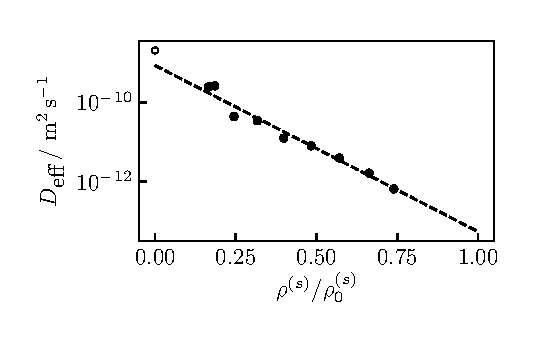
\includegraphics[width=\linewidth]{diffusion-fit-nano3}
  \caption{Binary diffusion constant for \ce{NaNO3}--\ce{H2O} solution.
  Solid points are experimental data from \cite{???} and the line is the numerical vft fit.}
\end{SCfigure}

\subsection{Liquid phase analysis II: concentration}

This is much simpler: before we had separate advection and diffusion terms, but with this choice of variables they merge into one.

\eqref{eq:species-continuity-advection-corrected} gives
\begin{equation}\label{eq:species-evolution-current}
  \begin{aligned}
    \frac{\partial \rho^{(i)}}{\partial t} &=
    - \vec{\nabla} \cdot \Big(
    \rho^{(i)} \vec{v} + \vec{j}^{(i)}
    \Big)
    \\
    &=
    - \vec{\nabla} \cdot \Big(
    (1 + \rho^{(i)} \Lambda^{(i)}) \vec{j}^{(i)}
    \Big)
    \qquad i \in \{f,s\}
  \end{aligned}
\end{equation}
Using \eqref{eq:density-lambda} we have
\begin{equation*}
  \begin{aligned}
    \vec{\nabla} \rho^{(i)} &=
    \rho \vec{\nabla} Y^{(i)} +
    Y^{(i)} \vec{\nabla} \rho \\
    &=
    \left(
    \rho + Y^{(i)} \frac{\partial \rho}{\partial Y^{(i)}}
    \right)
    \vec{\nabla} Y^{(i)}
    \\
    &=
    \left(
    \rho +
    Y^{(i)} \rho^2 \Lambda^{(i)}
    \right)
    \vec{\nabla} Y^{(i)} \\
    &=
    \left(
    1 +
    \rho^{(i)} \Lambda^{(i)}
    \right)
    \rho
    \vec{\nabla} Y^{(i)}
  \end{aligned}
\end{equation*}
so inserting this and \eqref{eq:ficks-law} into \eqref{eq:species-evolution-current} gives
\begin{equation}\label{eq:species-evolution-final}
  \begin{aligned}
    \frac{\partial \rho^{(i)}}{\partial t} &=
    \vec{\nabla} \cdot \Big(
    (1 + \rho^{(i)} \Lambda^{(i)})
    D_{\textrm{eff}} \rho \vec{\nabla} Y^{(i)}
    \Big) \\
    &=
    \vec{\nabla} \cdot \Big(
    D_{\textrm{eff}} \vec{\nabla} \rho^{(i)}
    \Big)
    \qquad i \in \{f,s\}
  \end{aligned}
\end{equation}

\subsection{Liquid phase boundary conditions}

The mass of each species inside the droplet is obtained from its concentration profile as
\begin{equation}
  m^{(i)}(t) = \int_{\mathbb{V}(t)} \rho^{(i)}(\vec{r},t) \, d^3|\vec{r}|
  \qquad i \in \{f,s\}
\end{equation}
where $\mathbb{V}$ is the volume of the droplet.
Differentiating this expression gives the mass flow into the droplet (of this species) as
\begin{equation}\label{eq:integral-continuity}
  \frac{d m^{(i)}}{dt} =
  \int_{\mathbb{V}(t)} \frac{\partial \rho^{(i)}}{\partial t} \, d^3|\vec{r}| +
  \int_{\partial \mathbb{V}(t)} \rho^{(i)} \, \vec{v}_{\partial \mathbb{V}(t)} \cdot d^2\vec{S}
  \qquad i \in \{f,s\}
\end{equation}
where $\vec{v}_{\partial \mathbb{V}(t)}$ is the velocity of the boundary and the vectorial surface element $d^2\vec{S}$ points in the direction of the outer normal vector.
\eqref{eq:integral-continuity} is the integral form of \eqref{eq:species-continuity}.
Note that solute does not leave the droplet, so all mass entering/leaving the droplet must be due to the solvent.
We write these conditions as
\begin{subequations}
  \begin{align}
    \frac{d m^{(s)}}{dt} &= 0 \\
    \frac{d m^{(f)}}{dt} &= \frac{d m}{dt}
  \end{align}
\end{subequations}
where $m = m^{(s)} + m^{(f)}$ is the total solute mass.
Inserting \eqref{eq:species-evolution-final} into \eqref{eq:integral-continuity} and applying Stokes' theorem to the volume integral gives
\begin{equation}
  \begin{aligned}
    \frac{d m^{(i)}}{dt} &=
    \int_{\partial \mathbb{V}(t)}
    (\rho^{(i)} (\vec{v}_{\partial \mathbb{V}(t)} - \vec{v}) - \vec{j}^{(i)})
    \cdot d^2\vec{S} \\
    &=
    \int_{\partial \mathbb{V}(t)}
    \rho^{(i)} (\vec{v}_{\partial \mathbb{V}(t)} - \vec{v}^{(i)})
    \cdot d^2\vec{S} \\
    &=
    \int_{\partial \mathbb{V}(t)}
    \Big(
    \rho^{(i)} \vec{v}_{\partial \mathbb{V}(t)} -
    (1 + \rho^{(i)} \Lambda^{(i)}) \vec{j}^{(i)}
    \Big)
    \cdot d^2\vec{S} \\
    &=
    \int_{\partial \mathbb{V}(t)}
    \Big(
    \rho^{(i)} \vec{v}_{\partial \mathbb{V}(t)} +
    (1 + \rho^{(i)} \Lambda^{(i)})
    D_{\textrm{eff}} \rho \vec{\nabla} Y^{(i)}
    \Big)
    \cdot d^2\vec{S} \\
    &=
    \int_{\partial \mathbb{V}(t)}
    \Big(
    \rho^{(i)} \vec{v}_{\partial \mathbb{V}(t)} +
    D_{\textrm{eff}} \vec{\nabla} \rho^{(i)}
    \Big)
    \cdot d^2\vec{S}
    \qquad i \in \{f,s\}
  \end{aligned}
\end{equation}
after making use of \eqref{eq:relative-mass-flux} in the latter step.
For our spherical droplets this becomes
\begin{equation}
  \begin{aligned}
    \frac{d m^{(i)}}{dt} &=
    4 \pi R^2
    \rho^{(i)}(R) \left( \frac{dR}{dt} - v^{(i)}(R) \right) \\
    &=
    4 \pi R^2
    \rho^{(i)}(R) \left(
    \frac{dR}{dt} +
    \left.\left(
    (1 + \rho^{(i)} \Lambda^{(i)})
    \frac{D_{\textrm{eff}}}{Y^{(i)}}
    \frac{\partial Y^{(i)}}{\partial r}
    \right)\right|_{r=R(t)}
    \right)
    \qquad i \in \{f,s\}
  \end{aligned}
\end{equation}
\begin{equation}
  \left. \frac{\partial Y^{(s)}}{\partial r} \right|_{r=R(t)} =
  -
  \frac{Y^{(s)}}{(1 + \rho^{(s)} \Lambda^{(s)}) D_{\textrm{eff}}(R)}
  \frac{dR}{dt}
\end{equation}
so
\begin{equation}
  \left. \frac{\partial \rho^{(s)}}{\partial r} \right|_{r=R(t)} =
  -
  \frac{\rho^{(s)}}{D_{\textrm{eff}}(R)}
  \frac{dR}{dt}
\end{equation}

We can simplify the above expression by using volume additivity.
\begin{equation*}
  \rho^{(f)} = Y^{(f)} \rho = (1 - Y^{(s)}) \rho = \rho - \rho^{(s)}
\end{equation*}
Reminder:
\begin{equation*}
  \rho =
  \rho^{(j)}_0 (1 - \rho^{(i)} \Lambda^{(i)})
  \qquad i,j \in \{f,s\}, \; j \ne i.
\end{equation*}
so we have
\begin{equation*}
  \frac{\partial \rho}{\partial \rho^{(i)}} =
  - \rho^{(j)}_0 \Lambda^{(i)}
  \qquad i,j \in \{f,s\}, \; j \ne i.
\end{equation*}
\begin{equation}
  \begin{aligned}
    \frac{d m}{dt} &=
    \frac{d m^{(f)}}{dt} \\
    &=
    4 \pi R^2
    \left(
    \rho^{(f)}(R)  \frac{dR}{dt} +
    \left[
    D_{\textrm{eff}}
    \frac{\partial \rho^{(f)}}{\partial r}
    \right]_{r=R(t)}
    \right) \\
    &=
    4 \pi R^2
    \left(
    \rho^{(f)}(R)
    \frac{dR}{dt} +
    \left[
    D_{\textrm{eff}}
    \left(
    \frac{\partial \rho}{\partial r} -
    \frac{\partial \rho^{(s)}}{\partial r}
    \right)
    \right]_{r=R(t)}
    \right) \\
    &=
    4 \pi R^2
    \left(
    \rho^{(f)}(R)
    \frac{dR}{dt} +
    \left[
    D_{\textrm{eff}}
    \left(
    1 - \frac{\partial \rho}{\partial \rho^{(s)}}
    \right)
    \frac{\partial \rho^{(s)}}{\partial r}
    \right]_{r=R(t)}
    \right) \\
    &=
    4 \pi R^2
    \left(
    \rho^{(f)}(R)
    \frac{dR}{dt} +
    \left[
    D_{\textrm{eff}}
    \left(
    1 - \rho^{(f)}_0 \Lambda^{(s)}
    \right)
    \frac{\partial \rho^{(s)}}{\partial r}
    \right]_{r=R(t)}
    \right) \\
    &=
    4 \pi R^2
    \left(
    \rho^{(f)}(R)
    \frac{dR}{dt} +
    \left( 1 - \rho^{(f)}_0 \Lambda^{(s)} \right)
    \rho^{(s)}(R)
    \frac{d R}{d t}
    \right) \\
    &=
    4 \pi R^2
    \left(
    \rho(R) - \rho^{(s)}(R) \rho^{(f)}_0 \Lambda^{(s)}
    \right)
    \frac{dR}{dt} \\
    &=
    4 \pi R^2
    \left(
    \rho_0^{(f)}(1 - \rho^{(s)}(R) \Lambda^{(s)}) - \rho^{(s)}(R) \rho^{(f)}_0 \Lambda^{(s)}
    \right)
    \frac{dR}{dt} \\
    &=
    4 \pi R^2 \rho_0^{(f)} \frac{dR}{dt}
  \end{aligned}
\end{equation}
or
\begin{equation}\label{eq:radial-evolution}
  \frac{dR}{dt} =
  \frac{1}{4\pi R^2 \rho^{(f)}_0} \frac{dm}{dt}.
\end{equation}

\subsection{Vapour phase analysis}

Ref.\ \cite{Sirignano2010} describes 6 vaporisation models that differ primarily by their treatment of heat/temp of fluid phase.
In order of increasing complexity these are:
\begin{enumerate}
\item const $T$ (enough to get $\Delta R^2 \propto t$ law)
\item Uniform but varying $T$
\item Conduction limit
\item Effective-conduction: treats internal circulation/convection of heat in an ad hoc manner
\item Vortex models
\item Navier-Stokes: in principle exact
\end{enumerate}

Some general notes:
\begin{itemize}
\item Generally, the thermal diffusivity of gas phase is much larger than that in the liquid phase (except near a critical point where physical properties become identical).
  Therefore transient liquid heating takes longer, and can often treat gas-phase as quasi-steady.
\item Internal heat circulation ignored in first three models above.
\item Gas has mass diffusion $\sim$ heat diffusion whereas in the liquid mass diffusion is much slower than heat diffusion
\end{itemize}

Key assumptions\todo{Also reference Slattery, \emph{Advanced transport phenomena}, (1999)}
\begin{enumerate}
\item Spherical symmetry
\item Quasi-steady
%\item Lack of convection currents: $\vec{j} = D \vec{\nabla} \rho$ omits $-\vec{u} \rho$ term.
\end{enumerate}

Starting from the continuity equation\todo{Insert key reference for this section is: Sirignano, W. A. \emph{Fluid dynamics and transport of droplets and sprays - Second edition} (2010).}:
\begin{equation}\label{eq:continuity-eqn}
  \frac{\partial \rho}{\partial t}
  + \vec{\nabla} \cdot \vec{j} = 0,
\end{equation}
where the divergence term in spherical coordinates is
\begin{equation}
  \vec{\nabla} \cdot \vec{j} =
  \frac{1}{r^2} \frac{\partial (r^2 \rho u)}{\partial r}
\end{equation}

We treat the vapour phase as a binary system of the water vapour and an ambient gas phase, $Y_W + Y_A = 1$%
\marginfootnote{We have a solute (\ce{NaCl} or \ce{NaNO3}) and an evaporating solvent (water), which unfortunately both have the initial $S$ so we need an alternative subscript to distinguish them.
  \textbf{What to use for the solute?}
  We use $W$ for the water component and $A$ for the ambient gas phase.
I find it more memorable to think of the subscript $A$ as standing for `atmosphere'.}[-2cm].
Absent any chemical reactions the total number of each species is conserved, so the continuity equation must be satisfied for each constituent:
\begin{equation}
  \frac{\partial (\rho Y_i)}{\partial t}
  + \vec{\nabla} \cdot \vec{j}_i = 0
\end{equation}
\begin{equation}
  \vec{\nabla} \cdot \vec{j}_i =
  \frac{1}{r^2} \frac{d}{dr} \left(
  r^2 \rho u Y_i - r^2 D_V \frac{d(\rho Y_i)}{dr}
  \right)
\end{equation}
here $D_V$ is understood as a binary diffusion constant%
\marginfootnote{The subscript $V$ stands for vapour.},
the same for both species, as there is no net flow of mass: the species merely mix.

If we assume relaxation in the vapour phase a quasi-steady vapour relaxation the time derivative in \eqref{eq:continuity-eqn} disappears leaving
\begin{equation}
  \frac{d}{dr} ( r^2 \rho u ) = 0
\end{equation}
which allows us to write
\begin{equation}\label{eq:mass-conservation}
  r ^2 \rho u = \textrm{constant} = -\frac{\dot{m}}{4\pi}.
\end{equation}
Similarly, for the species equation we have
\begin{equation}
  \frac{d}{dr} \left(
  r^2 \rho u Y_i - r^2 \rho D_V \frac{d Y_i}{dr}
  \right) = 0
  \label{eq:quasistatic-vapour-species-conservation}
\end{equation}
Using \eqref{eq:mass-conservation} we have
\begin{equation}\label{eq:ambient-gas-ode}
  -\frac{\dot{m}}{4\pi r^2 \rho D_V} Y_A - \frac{d Y_A}{dr} = 0.
\end{equation}
Defining
\begin{equation*}
  \phi_A(r) = -\frac{\dot{m}}{4\pi}
  \int_r^\infty  \frac{1}{\rho D_V (r')^2} \, dr'
\end{equation*}
\eqref{eq:ambient-gas-ode} becomes
\begin{equation}
  \frac{d\phi_A}{dr} Y_A - \frac{d Y_A}{dr} = 0.
\end{equation}
which can be integrated%
\marginfootnote{One way to do this integral involves multiplying through by the integrating factor $e^{-\phi_A(r)}$.}
giving
\begin{equation}
  Y_A(r) e^{-\phi_A(r)} = \textrm{constant}.
\end{equation}
Thus, we have
\begin{equation}
  \frac{Y_A(R)}{\displaystyle{\lim_{r \to \infty}} Y_A(r)} = e^{\phi_A(R)}.
\end{equation}
using the fact that $\displaystyle{\lim_{r \to \infty} \phi_A(r) = 0}$.
Transforming this in terms of the mass fraction of the water component $Y_F = 1 - Y_A$ we have
\begin{equation}
  \frac{1 - Y_F(R)}{1 - \displaystyle{\lim_{r \to \infty}} Y_F(r)} =
  1 + B = e^{\phi_A(R)},
\end{equation}
where we have defined the \emph{Spalding number} as
\begin{equation}
  %B(Y_F(R); \displaystyle{\lim_{r \to \infty}} Y_F(r)) =
  B =
  \frac{\displaystyle{\lim_{r \to \infty}} Y_F(r) - Y_F(R)}
       {1 - \displaystyle{\lim_{r \to \infty}} Y_F(r)}.
\end{equation}
Upon reinserting the definition of $\phi_A$ and rearranging we obtain the equation for the evaporation rate as
\begin{equation}
  \dot{m} = -
  \frac{4\pi \ln{(1 + B)}}
       {\int_r^\infty  \frac{1}{\rho D_V (r')^2} \, dr'}
\end{equation}
If we take the product $\rho D_V$ as a constant in the vapour phase, then we obtain the classic result for quasistatic evaporation:
\begin{equation}
  \dot{m} = - 4\pi \rho D_V R \ln{(1 + B)}.
\end{equation}

Empirical modification \cite{Abramzon1988}
\begin{align}
  \dot{m} &= - 2\pi \rho D_V R \; Sh^* \ln{(1 + B)}, \\
  \dot{m} &= - 2\pi \frac{k_F}{C_{pF}} R \; Nu^* \ln{(1 + B_T)} \\
  Sh^* &= 2 + \frac{(Sh_0 - 2)}{F_M} \\
  Nu^* &= 2 + \frac{(Nu_0 - 2)}{F_T} \\
  B_T &= \frac{C_{pF} (T_\infty - T(R))}{L(T_s) + Q_L / \dot{m}}.
\end{align}
I guess $Sh_0$ is a widely used fudge factor (to account for convection?), and this constitutes further corrections to it.

%% \subsection{Quasistatic expressions}

%% In the quasistatic limit the density profile relaxes instantaneously leaving only
%% \begin{equation}
%%   \rho_{hom}(t) = \lim_{D\to\infty}{\rho(r,t)}
%% \end{equation}
%% which inserted back into \eqref{eq:mass-equation} gives the droplet mass in this limit as
%% \begin{equation}
%%   m_{hom}(t) = 4\pi \rho_{hom}(t) \int_0^{R(t)} r^2 \, dr = \frac{4\pi R(t)^3}{3} \rho_{hom}(t)
%% \end{equation}
%% We can rearrange this relation for $R(t)$
%% \begin{equation}\label{eq:homogeneous-droplet-radius}
%%   R(t) = \left( \frac{3 \, m_{hom}(t)}{4\pi \rho_{hom}(t)} \right)^\frac{1}{3}
%% \end{equation}
%% where the corrections arise due to deviations from the homogeneous density profile $\Delta \rho = \rho(r) - \rho_{hom}$.
%% The solute mass fraction \eqref{eq:mass-fraction} reduces to
%% \begin{equation}\label{eq:homogeneous-solute-mass-fraction}
%%   \phi_{s,hom}(t) = \frac{m_s}{m_{hom}(t)}.
%% \end{equation}
%% In what follows we will drop the subscript $hom$ in all expressions

%% The trick to this method is realising that at short times the Kulmala coefficients remain approximately constant, leading to the following ODE and solution:
%% \begin{equation*}
%%   \frac{dR}{dt} = \frac{c}{R(t)} \quad \implies R(t) = \sqrt{R(0)^2 + 2ct}.
%% \end{equation*}

%% Differentiating \eqref{eq:homogeneous-droplet-radius} gives
%% \begin{equation}
%%   \frac{1}{3} \frac{d}{dt} \left( R^3 \right)
%%   = R^2 \frac{dR}{dt}
%%   = \frac{1}{4\pi} \frac{d}{dt} \left( \frac{m}{\rho} \right)
%%   = \frac{1}{4\pi} \left(
%%   \frac{1}{\rho} \frac{d m}{dt}
%%   - \frac{m}{\rho^2} \frac{d \rho}{dt}
%%   \right).
%% \end{equation}

%% We use \eqref{eq:homogeneous-solute-mass-fraction} to differentiate the density as
%% \begin{equation*}
%%   \frac{d\rho}{dt}
%%   = \rho'(\phi_s) \frac{d\phi_s}{dt}
%%   = -\rho'(\phi_s) \frac{m_s}{m^2} \frac{dm}{dt}
%%   = -\rho'(\phi_s) \frac{\phi_s}{m} \frac{dm}{dt}.
%% \end{equation*}
%% \begin{equation}
%%   \implies \quad \frac{dR}{dt}
%%   = \frac{1}{4\pi \rho} \left(
%%   1 + \phi_s \frac{\rho'(\phi_s)}{\rho}
%%   \right)
%%   \underbrace{\frac{1}{R^2} \frac{dm}{dt}}_{\propto 1/R}
%% \end{equation}

%% Giving the time integral from the ODE solution:
%% \begin{equation}
%%   \begin{aligned}
%%     R(t + \Delta t)
%%     &= \sqrt{R(t)^2 + \frac{1}{2\pi \rho R(t)}
%%       \left(
%%       1 + \phi_s \frac{\rho'(\phi_s)}{\rho}
%%       \right)
%%       \frac{dm}{dt} \Delta t} \\
%%     &= R(t) \left(
%%     1 + \frac{1}{4\pi \rho R(t)^3}
%%     \left(
%%     1 + \phi_s \frac{\rho'(\phi_s)}{\rho}
%%     \right)
%%     \frac{dm}{dt} \Delta t
%%     \right)
%%     + \mathcal{O}(\Delta t^2) \\
%%     &= R(t) \left(
%%     1 +
%%     \left(
%%     1 + \phi_s \frac{\rho'(\phi_s)}{\rho}
%%     \right)
%%     \frac{\dot{m}}{3m} \Delta t
%%     \right)
%%     + \mathcal{O}(\Delta t^2).
%%   \end{aligned}
%% \end{equation}

%% \subsection{Treating evaporation}
%% \subsection{Evolution of the concentration profile}
\subsection{Phase boundary}

At short times
\begin{subequations}
  \begin{align}
    R(t) &\simeq \sqrt{R(t=0)^2 + A t} \qquad \\
    \implies \; \frac{dR}{dt} &\simeq \frac{A}{2R}.
  \end{align}
\end{subequations}
From \eqref{eq:radial-evolution}
\begin{equation}
  \begin{aligned}
  \frac{dR}{dt} &=
  -\frac{1}{4\pi R^2 \rho^{(f)}_0}
  2\pi Sh \rho_V D_V R \ln{(1 + B)} \\
  &=
  -\frac{Sh}{2 R \rho^{(f)}_0}
  \rho_V D_V \ln{(1 + B)} =
  \frac{A}{2 R} \\
  Sh &= \frac{A \rho^{(f)}_0}{\rho_V D_V \ln{(1+B)}}
  \end{aligned}
\end{equation}
so we can work out the empirical correction if we know the initial $\dot{R}$ from fitting the parameter $A$.

The steady state heat flux through the droplet boundary in the steady state is \cite{Kulmala1993,Rovelli2016}
\begin{equation}
  Q = Q_R - h \frac{dm^{(f)}}{dt} + 4\pi R K (T(R) - T_\infty)
\end{equation}
where $Q_R$ is the excess heat flux of radiation over absorption, $h$ is the vapour enthalpy of the evaporating solvent, and $K$ is the thermal conductivity of the gas phase.
Neglecting the droplet heat capacity and the effect of radiation gives the temperature difference between
the droplet surface and the ambient temperature as \cite{Kulmala1993,Rovelli2016}
\begin{equation}
  T(R) - T_\infty = \frac{L}{4\pi R K} \frac{dm^{(f)}}{dt}
\end{equation}

The mass fraction at the surface, and thus $B$, is determined through the Clausius-Clapeyron relation.
We have
\begin{equation}\label{eq:Clausius-Clapeyron}
  \frac{d P}{dT} = \frac{L}{T \Delta v}
\end{equation}
where $L$ is the specific latent heat of evaporation, and $\Delta v$ is the specific volume change between the liquid and vapour
\begin{equation}
  \Delta v
  \equiv v_g - v_l
  \sim v_g
  = \frac{RT}{P}
\end{equation}
where the approximation holds for the gas-liquid transition because $v_l \ll 1$ and we used the ideal gas law in the last step.
Taking $L$ as constant with respect to $T$ \eqref{eq:Clausius-Clapeyron} becomes
\todo{We use $R$ for both the droplet radius and the molar gas constant, so we need to change the symbol for the radius to e.g.\ $a$.}
\begin{equation}
  \int_{P_1}^{P_2} \frac{d P}{P} =
  \frac{L}{R} \int_{T_1}^{T_2} \frac{dT}{T^2}
\end{equation}
giving
\begin{equation}\label{eq:Clausius-Clapeyron-pressure-difference-mono}
  \begin{aligned}
    P_2 &=
    P_1 \exp{\left( \frac{L}{R} \left(\frac{1}{T_1} - \frac{1}{T_2} \right) \right)} \\
    &=
    P_1 \exp{\left( \frac{L}{R} \frac{T_2 - T_1}{T_1 T_2} \right)}
  \end{aligned}
\end{equation}
though for a binary mixture $P_i$ represents the partial pressures of the evaporating components,
where the partial pressure is determined from the solvent activity by
\begin{subequations}
  \begin{align}
    P_1 &= a_w(Y^{(f)}) P_{eq} \\
    P_2 &= P(R^-) \\
    T_1 &= T_\infty
  \end{align}
\end{subequations}
so \eqref{eq:Clausius-Clapeyron-pressure-difference-mono} becomes
\todo{We use lower case $p$ to mean pressure in the rest of the thesis, so we should change $P \to p$ here too.}
\begin{equation}\label{eq:Clausius-Clapeyron-pressure-difference-binary}
  P(R^-) =
  a_w(Y^{(f)}) P_{eq}
  \exp{\left( \frac{L}{R} \frac{T(R) - T_\infty}{T(R) T_\infty} \right)}
\end{equation}
Finally, the molar fraction of the fluid component at the surface is obtained from
\begin{equation}
  P(R^-) = X^{(f)}(R^+) P
\end{equation}
giving the mass fraction as
\begin{equation}
  \begin{aligned}
    Y^{(f)}(R^+) &=
    \frac{X^{(f)}(R^+) W^{(f)}}{X^{(f)}(R^+) W^{(f)} + X^{(g)} W^{(g)}} \\
    &=
    \frac{X^{(f)}(R^+) W^{(f)}}{X^{(f)}(R^+) W^{(f)} + (1 - X^{(f)}(R^+)) W^{(g)}}.
  \end{aligned}
\end{equation}
where $W^{(f)}$ and $W^{(g)}$ are the molar masses of the solvent and air components respectively.

%% Taking into account the latent heat across the phase boundary, we expect
%% \begin{equation}
%%   \frac{\rho^{(f)}(R^+)}{\rho^{(f)}(R^-)} =
%%   e^{-\beta L}
%% \end{equation}
%% where $T$ is the temperature at the droplet surface, $L$ is the latent heat of vaporisation (per unit mole) and $R$ is the molar gas constant.
%% So the mass fraction ratios become
%% \begin{equation}
%%   \begin{aligned}
%%     \frac{Y^{(f)}(R^+)}{Y^{(f)}(R^-)} &=
%%     \frac{\rho^{(f)}(R^+)}{\rho(R^+)}
%%     \frac{\rho(R^-)}{\rho^{(f)}(R^-)} \\
%%     &=
%%     \frac{\rho(R^-)}{\rho_V}
%%     e^{-\beta L}
%%   \end{aligned}
%% \end{equation}
%% assuming $\rho(R+) = \rho_V$.

%% \begin{equation*}
%%   \ln{(1 + B)} = B + \mathcal{O}(B^2)
%% \end{equation*}
%% recall:
%% \begin{equation*}
%%   \begin{aligned}
%%     1 + B &=
%%     \frac{1 - Y_F(R^+)}{1 - \displaystyle{\lim_{r \to \infty}} Y_F(r)} \\
%%     &=
%%     \frac{1 - \frac{\rho_V}{\rho(R^-)}
%%       e^{-\beta L} Y_F(R^-)}{1 - \displaystyle{\lim_{r \to \infty}} Y_F(r)} \\
%%     &=
%%     1 - \frac{\rho_V}{\rho(R^-)} e^{-\beta L} Y_F(R^-)
%%   \end{aligned}
%% \end{equation*}
%% for $\lim_{r \to \infty} Y_F(r) = 0$ in the final step

%% So we have
%% \begin{equation*}
%%   \begin{aligned}
%%     \frac{dR}{dt} &=
%%     -\frac{Sh}{2 R \rho^{(f)}_0}
%%     \rho_V D_V B + \mathcal{O}(B^2) \\
%%     &=
%%     -\frac{Sh}{2 R \rho^{(f)}_0}
%%     \rho_V D_V B + \mathcal{O}(B^2)
%%   \end{aligned}
%% \end{equation*}

\section{Implementation and results}

\todo{Figure of state point evolution (boundary concentration and temperature) for \ce{NaCl} droplets.
  Indicate point where 50\% have nucleated, with bars for the upper and lower bounds.
  These should show a more-or-less fixed final boundary concentration.}

For \ce{NaCl} the agreement is very good, as a step function in the nucleation rates seems to hold.
However, the theory predicts similar behaviour for \ce{NaNO3} which is not seen in the experiments.
The cause of this breakdown is unknown.

At long times the radial evolution shows some discrepancy with the experiments, suggesting our semi-empirical treatment of evaporation breaks down.

\section{Discussion}


Classical nucleation theory with physically plausible parameters, seems to work well for \ce{NaCl} solutions but not for \ce{NaNO3}.
In both cases CNT predicts nucleation essentially after a threshold surface saturation is reached, whereas experiments show nucleation in \ce{NaNO3} has stochastic behaviour.
The discrepancy is either due to the assumptions entering into our evolution equations, leading to incorrect trajectories entering the CNT calculation, or CNT itself does not predict accurate nucleation kinetics for this solution.
We consider each of these possibilities in turn.

It is unlikely to be due to the trajectories being incorrect: even varying the most poorly estimated parameter for \ce{NaNO3}, the surface tension, does not change the CNT prediction.
Because of the sensitivity of CNT on parameters, it would require a remarkable degree of fine tuning to fit CNT model with any physically plausible parameters.
It's possible nucleation of \ce{NaNO3} occurs via a more complex kinetic pathway, e.g.\ multiple steps \cite{?,?,?}.
Alternatively, the experimental nucleation could be occurring via heterogeneous nucleation (e.g.\ impurities in the sample).
This is unlikely however, as the experiments can maintain the same salt sample and follow the single trajectory and it will still show the same stochastic behaviour.
Impurities are not likely to be in the solvent, or we would likely see the same phenomenon in \ce{NaNO3} nucleation.

Our evaporation model is rather crude, though it seems to qualitatively show the right behaviour.
It's possible that our assumption of pure Fickian diffusion oversaturates the concentration at the boundary.
To go beyond this one would have to introduce more sophisticated kinetics beyond Fickian diffusion.
An option would be to relax the assumption that the temperature of the droplet is constant, as convection effects could play a key role in mixing the solution.
Solving the Navier-Stokes equations would be essentially exact, though expensive route to include this.
Less expensive would be to use vortex models or effective-conduction models which treat the internal circulation/convection of heat in an ad hoc manner.

\section*{Appendix: Numerical implementation}

$\rho(r)$ will later be discretised into the density at equally spaced points of separation $\Delta r$, so it is natural to think of it as a vector of points $\vec{\rho} = \{\rho(0), \rho(\Delta r), \rho(2 \Delta r), \cdots, \rho(1)\} = \{\rho_1, \cdots, \rho_N\}$ so we will use the notation $\vec{\rho}$ from
now on to mean $\rho(r)$.

To integrate a timestep $\Delta t$ we use the Crank-Nicolson \cite{Crank1947} method where the time derivative for integration is taken as the average of the instantaneous derivatives at the start and end of integration.
This is essentially a midpoint method, but requires a bit of linear algebra to solve as we do not know the value of $\partial \vec{\rho} / \partial t$ until we also know $\vec{\rho}$.
Starting from
\begin{equation}
  \frac{\partial \vec{\rho}}{\partial t} =
  \lim_{\Delta t \to 0} \frac{\vec{\rho}(t + \Delta t) - \vec{\rho}(t)}{\Delta t}
\end{equation}
after discretising we obtain
\begin{equation}
  \frac{\vec{\rho}(t + \Delta t) - \vec{\rho}(t)}{\Delta t}
  =
  \frac{1}{2}
  \left(
  \left. \frac{\partial \vec{\rho}}{\partial t} \right|_{t + \Delta t}
  +
  \left. \frac{\partial \vec{\rho}}{\partial t} \right|_t
  \right)
  + \mathcal{O}(\Delta t^2).
\end{equation}
The main advantage of this scheme over more simple schemes (e.g. forward Euler method where we just take the initial $\partial \vec{\rho} / \partial t$) is that the error is of order $\Delta t^2$; this ensures rapid convergence to the correct solution with small integration steps.

Labelling $\vec{\rho}(t) = \vec{\rho}_n$ and $\vec{\rho}(t + \Delta t) = \vec{\rho}_{n+1}$, the goal is to make progressively better guesses for $\vec{\rho}_{n+1}$.
We label the $k^\textrm{th}$ approximation for $\vec{\rho}_{n+1}$ as $\vec{\rho}_{n+1}^{(k)}$ where the initial guess is $\vec{\rho}_{n+1}^{(1)} = \vec{\rho}_n$, and derive an iterative formula to find $\vec{\rho}_{n+1}^{(k+1)}$ which converges to $\vec{\rho}_{n+1}$ in the limit $k \to \infty$, although in practice only a few iterations should be enough to achieve an approximate solution.
Using the Crank-Nicolson scheme we write
\begin{equation}
  \frac{\vec{\rho}_{n+1}^{(k+1)} - \vec{\rho}_n}{\Delta t}
  =
  \frac{\vec{\rho}_{n+1}^{(k)} + \delta \vec{\rho}_{n+1}^{(k)} - \vec{\rho}_n}{\Delta t}
  =
  \frac{1}{2}
  \left(
  \frac{\partial (\vec{\rho}_{n+1}^{(k)} + \delta \vec{\rho}_{n+1}^{(k)})}{\partial t}
  +
  \frac{\partial \vec{\rho}_n}{\partial t}
  \right)
\end{equation}
This is complicated by the fact that $\rho(r)$ depends on $R(t)$ making this equation nonlinear as it couples with the evolution of $R(t)$.
As such, the above equation implicitly involves terms $R_{n+1}^{(k)} + \delta R_{n+1}^{(k)}$.
To find the form of the right-hand side we expand in powers of $\delta \vec{\rho}_{n+1}^{(k)}$ and $\delta R_{n+1}^{(k)}$ retaining only those linear.
Doing this we find...
\begin{equation}
  \frac{\vec{\rho}_{n+1}^{(k)} + \delta \vec{\rho}_{n+1}^{(k)} - \vec{\rho}_n}{\Delta t}
  =
  F_\rho^{(k)} (\vec{\rho}_n, \vec{\rho}_{n+1}^{(k)}, R_n, R_{n+1}^{(k)}) +
  G_\rho^{(k)} (\vec{\rho}_{n+1}^{(k)}, R_{n+1}^{(k)}) \delta \vec{\rho}_{n+1}^{(k)} +
  H_\rho^{(k)} (\vec{\rho}_{n+1}^{(k)}, R_{n+1}^{(k)}) \delta R_{n+1}^{(k)}
\end{equation}
where the functions $F_\rho^{(k)},G_\rho^{(k)},H_\rho^{(k)}$ are long and not particularly illuminating so we omit their explicit form for the sake of brevity.
Importantly $F_\rho^{(k)},G_\rho^{(k)},H_\rho^{(k)}$ are functions of known variables and $\delta \vec{\rho}_{n+1}^{(k)}, \delta R_{n+1}^{(k)}$.
We can do a similar expansion for the evolution of the boundary, i.e.\
\begin{equation}\label{eq:discrete-evolution-rho}
  \frac{R_{n+1}^{(k)} + \delta R_{n+1}^{(k)} - R_n}{\Delta t}
  =
  \frac{1}{2}
  \left(
  \frac{\partial (R_{n+1}^{(k)} + \delta R_{n+1}^{(k)})}{\partial t}
  +
  \frac{\partial R_n}{\partial t}
  \right)
\end{equation}
and we perform the same expansion as before to obtain something of in the form of
\begin{equation}\label{eq:discrete-evolution-R}
  \frac{R_{n+1}^{(k)} + \delta R_{n+1}^{(k)} - R_n}{\Delta t}
  =
  F_R^{(k)} (\vec{\rho}_n, \vec{\rho}_{n+1}^{(k)}, R_n, R_{n+1}^{(k)}) +
  G_R^{(k)} (\vec{\rho}_{n+1}^{(k)}, R_{n+1}^{(k)}) \delta \vec{\rho}_{n+1}^{(k)} +
  H_R^{(k)} (\vec{\rho}_{n+1}^{(k)}, R_{n+1}^{(k)}) \delta R_{n+1}^{(k)}
\end{equation}
with new functions $F_R^{(k)},\vec{G}_R^{(k)},H_R^{(k)}$ which are also of known variables.
In all likelyhood, these only depend on the density of the solute at the boundary.
We can combine equations \eqref{eq:discrete-evolution-rho} and \eqref{eq:discrete-evolution-R} into a single matrix equation, i.e.
\begin{equation}
  \begin{pmatrix}
    \vec{G}_\rho^{(k)} \Delta t - 1 & H_\rho^{(k)} \Delta t \\
    G_R^{(k)} \Delta t & H_R^{(k)} \Delta t - 1
  \end{pmatrix}
  \begin{pmatrix}
    \delta \vec{\rho}_{n+1}^{(k)} \\
    \delta R_{n+1}^{(k)}
  \end{pmatrix}
  =
  \begin{pmatrix}
    \vec{\rho}_{n+1}^{(k)} - \vec{\rho}_n^{(k)} -
    F_\rho^{(k)} (\vec{\rho}_n, \vec{\rho}_{n+1}^{(k)}, R_n, R_{n+1}^{(k)})
    \Delta t
    \\
    R_{n+1}^{(k)} - R_n^{(k)} -
    F_R^{(k)} (\vec{\rho}_n, \vec{\rho}_{n+1}^{(k)}, R_n, R_{n+1}^{(k)})
    \Delta t
  \end{pmatrix}.
\end{equation}
The terms on the right-hand side of this matrix equation are called th eresiduals, and the left-hand side consists of the (Jacobian) matrix and the vector of unknowns.
The solution is found by inverting the matrix.
If we write $\vec{x}_n = (\vec{\rho}_n, R_n)^T$ we have
\begin{equation}
  \delta \vec{F} \cdot \delta \vec{x}_{n+1}^{(k)} =
  \vec{F}(\vec{x}_n, \vec{x}_{n+1}^{(k)}
\end{equation}
where $\vec{F}(\vec{x}_n, \vec{x}_{n+1}^{(k)}) = \vec{x}_{n+1}^{(k)} - \vec{x}_n - \Delta t (F_\rho^{(k)} (\vec{x}_n, \vec{x}_{n+1}^{(k)}), F_R^{(k)} (\vec{x}_n, \vec{x}_{n+1}^{(k)}))^T$ giving solution
\begin{equation}
  \delta \vec{x}_{n+1}^{(k)} =
  (\delta \vec{F}^{(k)})^{-1} \cdot \vec{F}(\vec{x}_n, \vec{x}_{n+1}^{(k)}).
\end{equation}
We iterate this inversion procedure until some stop criterion is met (i.e.\ we find $\vec{x}_{n+1}$ to some desired accuracy), giving the final solution after $k_{stop}$ iterations:
\begin{equation}
  \vec{x}_{n+1} =
  \vec{x}_n + \sum_{k=1}^{k_{stop}}
  (\delta \vec{F}^{(k)})^{-1} \cdot \vec{F}(\vec{x}_n, \vec{x}_{n+1}^{(k)})
  + \mathcal{O}(\Delta t^2).
\end{equation}
A sensible stop criterion is that the residuals $F(\vec{x}_n, \vec{x}_{n+1}^{(k)}$ fall to some small value close to zero, meaning $\delta\vec{x}^{(k+1)}$ is small and we are sufficiently close to the true $\vec{x}_{n+1}$.
Note that the true $\vec{x}_{n+1}$ is not `true' in the sense that it is the exact result, i.e. $(\rho(t + \Delta t), R(t + \Delta t))^T$, but rather true in the sense that it is the correct result predicted by this method (i.e. to $\mathcal{O}(\Delta t^2)$ accuracy).

\end{document}
